Il capitolo ha lo scopo di illustrare i concetti e i metodi statistici che stanno alla base delle elaborazioni effettuate.

In primo luogo si riporteranno le definizioni degli indici statistici e dei valori comunemente utilizzati in qualsiasi analisi statistica di base.

Successivamente saranno spiegati alcuni metodi statistici atti a individuare le caratteristiche della serie di dati in esame.

\section{Statistica descrittiva}
\label{sec:stat_desc}
La statistica descrittiva è una caratterizzazione quantitativa dei dati, condotta attraverso il calcolo di alcuni parametri che sintetizzano le più importanti caratteristiche statistiche dei dati \cite{book}. Come già spiegato nel \autoref{ch:3}, questa analisi fornisce alcune caratteristiche intrinseche della serie di dati che si riferiscono alla lunghezza e alla completezza della serie e alla distribuzione dei dati mancanti nella serie stessa.

Altri parametri utili per descrivere statisticamente una serie di dati si suddividono in indici di posizione, indici di dispersione e indici di forma.\\

\textit{Nota: le definizioni presenti in questa sezione, se non espressamente indicato, sono estratte da \cite{ross2008probabilita}}.

\subsection{Indici di posizione}
\label{sec:ind_pos}
Gli indici di posizione danno informazioni relative alla posizione dei dati sulla scala dei numeri, cioè indicano l'ordine di grandezza dei valori assunti dai dati \cite{book}.
\subsubsection{Media}
La media $\bar{x}$ di una serie di $n$ misurazioni $x_{1}, x_{2},\dots, x_{n}$ è definita come:

\begin{equation}
\bar{x}\coloneqq\frac{1}{n}\sum_{i=1}^{n}x_{i}
\end{equation}

\subsubsection{Percentili}
Dato il numero intero $k$ compreso tra 0 e 100 e data una serie di dati, si definisce $k$-esimo percentile il valore maggiore o uguale al $k$ percento dei dati.

Tra i percentili, i più rilevanti sono:
\begin{itemize}
	\item 25° percentile, detto anche \textit{primo quartile};
	\item 50° percentile, detto anche \textit{secondo quartile} o \textit{mediana};
	\item 75° percentile, detto anche \textit{terzo quartile}.
\end{itemize}

A differenza della media, la mediana è un indice di posizione robusto perché non risente della presenza di eventuali \textit{outliers} \cite{book} (per la definizione, si veda \autoref{sec:outliers}).

\subsection{Indici di dispersione}
Gli indici di dispersione descrivono quanto i dati siano concentrati o dispersi rispetto ai valori determinati dagli indici di posizione e quindi indicano la variabilità dei dati \cite{ross2008probabilita}.
\subsubsection{Varianza}
La varianza $s^{2}$ di una serie di $n$ misurazioni $x_{1}, x_{2},\dots, x_{n}$ di media $\bar{x}$ è definita come:

\begin{equation}
s^{2}\coloneqq\frac{1}{n-1}\sum_{i=1}^{n}(x_{i}-\bar{x})^{2}
\end{equation}

\subsubsection{Scarto quadratico medio}
Lo scarto quadratico medio, o deviazione standard, $s$ di una serie di $n$ misurazioni $x_{1}, x_{2},\dots, x_{n}$ di media $\bar{x}$ è la radice quadrata della varianza:

\begin{equation}
s\coloneqq\sqrt{\frac{1}{n-1}\sum_{i=1}^{n}(x_{i}-\bar{x})^{2}}
\end{equation}

\subsubsection{Coefficiente di variazione}
Il coefficiente di variazione $CV$, o deviazione standard relativa, di una serie di $n$ misurazioni $x_{1}, x_{2},\dots, x_{n}$ di media $\bar{x}$ è definito come \cite{brown2002statistics}:

\begin{equation}
CV\coloneqq\frac{s}{\bar{x}}
\end{equation}

Questo indice è di particolare utilità qualora si volessero confrontare le variabilità di diverse serie di dati perché non è dipendente dalla media dei dati, come invece avviene se si considera la deviazione standard. 



\subsection{Indici di forma}
Gli indici di forma danno informazioni riguardo alla forma della distribuzione dei dati \cite{book}.

\subsubsection{Indice di asimmetria}
L'indice di asimmetria, o \textit{skewness}, $\gamma$ di una serie di $n$ misurazioni $x_{1}, x_{2},\dots, x_{n}$ di media $\bar{x}$ è definito come:

\begin{equation}
\gamma=\frac{\frac{1}{n}\sum_{i=1}^{n}(x_{i}-\bar{x})^{3}}{[\frac{1}{n}\sum_{i=1}^{n}(x_{i}-\bar{x})^{2}]^{3/2}}
\end{equation}

Se l'indice assume valori positivi, si avrà una maggiore frequenza dei valori inferiori alla media e, viceversa, se l'indice è negativo si avrà una minore frequenza dei valori inferiori alla media. Se la distribuzione dei dati è simmetrica, invece, l'indice di asimmetria sarà pari a 0 \cite{book}.

\subsection{\textit{Box plot}}
\label{subsec:boxplot_th}

Le caratteristiche di una serie di dati possono essere descritte anche attraverso il grafico chiamato \textit{box plot} (o \textit{box-and-whisker plot}) (\autoref{fig:th_boxplot}). Esso evidenzia la mediana con una barra centrale e i quartili (corrispondenti al 25° e al 75° percentile) come un rettangolo (\textit{box}). Il rettangolo, quindi, include il 50\% dei dati, ovvero il cosiddetto scarto interquartile. I due segmenti esterni, detti baffi (\textit{whiskers}), includono tutti i valori ad eccezione di quelli più estremi che sono invece rappresentati con dei pallini (come indicato nella \autoref{sec:outliers}, saranno considerati possibili \textit{outliers}) \cite{brown2002statistics}.

\begin{figure}[h]
	\fbox{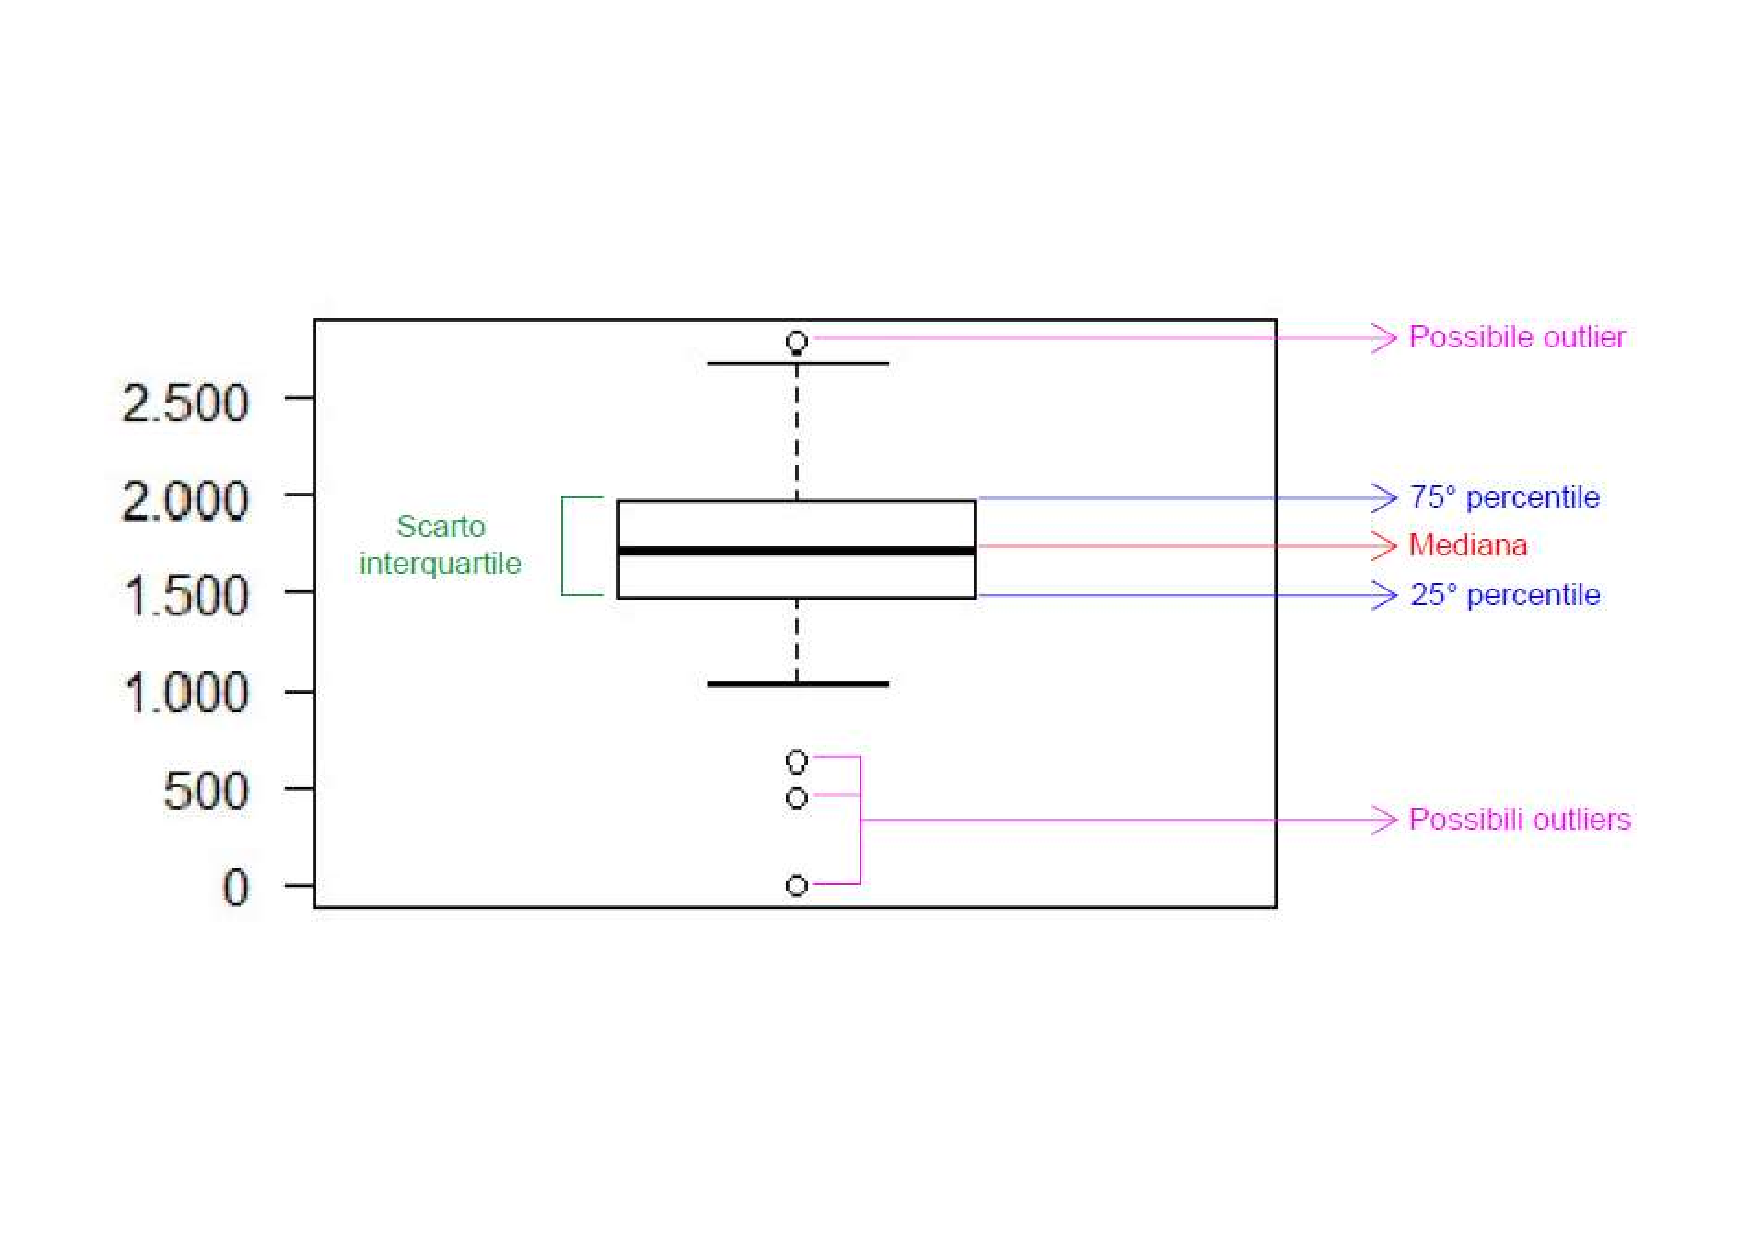
\includegraphics[width=\linewidth]{th_boxplot}}	\centering
	\caption{Esempio di \textit{box plot}}
	\label{fig:th_boxplot}
\end{figure} \pagebreak

\section{\textit{Outliers}}
\label{sec:outliers}
Gli \textit{outliers}, o valori anomali, sono quei valori che si discostano marcatamente dagli altri valori della serie di dati. Per evitare di trarre conclusioni errate, prima di procedere all'analisi statistica è opportuno valutare quali dati siano da considerarsi \textit{outliers} e come trattarli. 
Ci sono più metodi per definire, individuare e trattare gli \textit{outliers} e non c'è un criterio per stabilire quale tra questi sia il migliore. Una volta scelto uno di questi metodi, è importante indicarlo e descriverlo, in modo da garantire la massima trasparenza e permettere una piena comprensione dell'analisi da parte di un eventuale lettore \cite{outliers}.

Nel caso in esame, si è innanzitutto fatta una distinzione tra due tipi di \textit{outliers}:
\begin{itemize}
	\item \textbf{\textit{Error outliers}}: dati che si trovano a una certa distanza dagli altri poiché sono il risultato di misure non accurate. Per esempio possono essere dati che derivano da errori di campionamento, errori nella manipolazione dei dati, errori di calcolo o dati che sono al di fuori del possibile intervallo di valori.
	\item \textbf{\textit{Interesting outliers}}: misure accurate che giacciono a una certe distanza dagli altri dati e che contengono informazioni inattese ma importanti.
\end{itemize}

\subsection{Procedura di identificazione e di trattamento degli \textit{outliers}}
\label{subsec:procedura_outliers}
Un metodo semplice per identificare gli \textit{outliers} è l'utilizzo dei \textit{box plot}. Come già mostrato nella \autoref{fig:th_boxplot}, i possibili \textit{outliers} sono i punti agli estremi del grafico. In particolare, essi rappresentano i valori che giacciono al di fuori dell'intervallo pari a 1,5 volte lo scarto interquartile\footnote{Come indicato nella documentazione di R: \url{https://www.rdocumentation.org/packages/graphics/versions/3.5.1/topics/boxplot}}.

I dati così individuati sono dei potenziali \textit{error outliers} o potenziali \textit{interesting outliers}. 

Nel primo caso, bisogna valutare se essi siano effettivamente valori anomali. \`E quindi necessario determinare la causa dell'anomalia: se c'è un errore nella raccolta e registrazione del dato, allora esso è un \textit{error outlier}, se invece la causa non è chiara, esso diventa un \textit{interesting outlier}.

Stabilito quali dati siano \textit{error outliers}, si procede modificando il valore, sostituendolo con quello corretto, oppure rimuovendolo. La decisione deve essere presa dall'esperto del dominio in cui si opera e deve essere motivata.

A questo punto, si valutano i potenziali \textit{interesting outliers} (quelli individuati fin dall'inizio e quelli che si è stabilito non fossero \textit{error outliers}). Anche in questo caso, l'esperto di dominio, grazie alle sue competenze e consapevole del fine ultimo dell'analisi, studia i valori anomali e decide se conservarli, modificarli o eliminarli, specificando sempre la motivazione della scelta \cite{outliers}.

\section{Dati mancanti}
\label{sec:NA}
Quando si raccolgono e registrano i dati di una \textit{time series}, capita spesso che si abbia a che fare con alcuni dati mancanti. Il dato può mancare per diversi motivi: non è stato misurato, è stato misurato ma è andato perso, è stato misurato ma è considerato inutilizzabile \cite{Moritz2015ComparisonOD}. 

Una serie contenente valori mancanti può far nascere dei problemi perché, per alcune analisi, sono richieste serie complete di dati. Di conseguenza, è opportuno valutare quale sia il metodo migliore per risolvere questi problemi, in base al tipo di analisi che si vuole condurre. Se si volessero confrontare due serie di dati, sarebbe necessario avere dati campionati in maniera sincrona (per esempio negli stessi giorni dell'anno), se si volesse invece fare un'analisi di frequenza, servirebbe una frequenza di campionamento costante, a intervalli regolari.

Si definiscano, innanzitutto, i diversi tipi di \textit{missing data} \cite{Moritz2015ComparisonOD}:
\begin{itemize}
	\item \textbf{MCAR - \textit{Missing Completely At Random}}: la posizione dei dati mancanti non segue un meccanismo sistematico ma è completamente casuale. Questo implica che la probabilità che una certa osservazione sia mancante è indipendente dal valore delle altre variabili e che tale probabilità è indipendente anche dal valore dell'osservazione stessa. Nel caso in cui si abbia una \textit{time series} univariata (ovvero di una sola variabile), la probabilità che una certa osservazione sia mancante è indipendente dall'istante temporale dell'osservazione nella serie.
	\item \textbf{MAR - \textit{Missing At Random}}: la probabilità che un'osservazione sia mancante è indipendente dal valore dell'osservazione stessa ma è dipendente dalle altre variabili (compresa la variabile temporale). Nelle \textit{time series} univariate, tale probabilità dipende dall'istante temporale dell'osservazione.
	\item \textbf{NMAR - \textit{Not Missing At Random}}: la probabilità che un'osservazione sia mancante dipende dal valore della variabile stessa e potrebbe dipendere anche da altre variabili.
\end{itemize}

\subsection{Tecniche di trattamento dei dati mancanti}
\label{subsec:NAhandling}
Di seguito saranno elencati alcuni metodi che possono essere applicati per risolvere i problemi legati alla presenza di dati mancanti \cite{article}.

\paragraph*{\textit{Case deletion}}
Questo metodo consiste nell'eliminare i casi in cui ci sono dati mancanti e quindi significa che si esegue un'analisi dei casi completi. Per esempio, con riferimento ai dati trattati in questo lavoro, bisognerebbe considerare esclusivamente le misurazioni dei giorni in cui si ha il dato per ogni parametro.

\paragraph*{\textit{Pairwise deletion}} 
Il metodo prevede l'eliminazione dei casi incompleti ma esclusivamente se relativi al tipo di analisi che si sta conducendo. Questi casi potranno essere comunque utilizzati per altre analisi. Per fare un esempio, si pensi ad un'analisi che coinvolga il rapporto tra BOD\textsubscript{5} e COD: verranno considerati solamente i giorni in cui si hanno le misure di entrambi i parametri, ma i giorni scartati potranno essere utilizzati per altre analisi.

\paragraph*{\textit{Mean substitution}}
I dati mancanti vengono sostituiti con il valore della media di tutti i dati. In alternativa la media può essere calcolata facendo una aggregazione dei dati. Per esempio, si calcola la media settimanale e il suo valore viene assegnato ai dati mancanti della settimana considerata.

\paragraph*{Imputazione per regressione}
Il processo di imputazione consiste nella sostituzione dei dati mancanti con un valore stimato. In questo caso, l'imputazione viene fatta sostituendo i valori mancanti tramite un'equazione di regressione.

\paragraph*{\textit{Last observation carried forward}}
Ogni dato mancante viene rimpiazzato con il valore dell'ultima osservazione.

\paragraph*{\textit{Maximum likelihood}}
Questo metodo si applica quando ci sono alcuni dati mancanti ma la serie è relativamente completa. I dati mancanti vengono sostituiti utilizzando la distribuzione di probabilità delle altre variabili.

\paragraph*{Imputazione multipla}
L'imputazione viene condotta con un modello di regressione contenente una componente casuale che cerca di mantenere la varianza originale dei dati. Il processo viene ripetuto $m$ volte, ottenendo quindi $m$ possibili nuove serie di dati. Ciascuna di esse viene analizzata con le procedure statistiche standard per le serie complete e, combinando i risultati ottenuti, si ottiene il valore finale da inserire al posto del dato mancante.

\section{Media mobile}
\label{sec:MA}
La curva della media mobile (\textit{moving average}) permette di smussare le variazioni estreme nel grafico della \textit{time series} e di evidenziare eventuali trend e ciclicità. Per calcolare la media mobile, si considera una periodo mobile di $m$ valori (che, nel caso di \textit{time series}, rappresentano giorni o anni), preferibilmente dispari. Preso il punto centrale del periodo, si calcola la media aritmetica del valore del punto stesso e dei valori interni al periodo che lo precedono e lo seguono. Il risultato è il valore dell'ordinata del punto della curva della media mobile che corrisponde all'ascissa del punto centrale considerato in partenza.
La media mobile di un periodo di $m$ valori applicata a una serie di $n$ valori restituisce una serie di lunghezza $n-2k$, dove $k=(m-1)/2$:
\begin{equation}
y_{i}=\frac{1}{m}\sum_{j=i-k}^{i+k}x_{j};\;con\;	i=k+1,k+2,\dots,(n-k)
\end{equation}

Sebbene dal punto di vista matematico l'ampiezza $m$ del periodo mobile possa essere scelta a piacere, per avere risultati significativi è necessario che essa sia sufficientemente piccola rispetto alla lunghezza $n$ delle serie di dati \cite{MA}.

\section{Componenti di una \textit{time series}}
\label{sec:componenti}
Una \textit{time series} può essere considerata come la somma di tre componenti \cite{book}:
\begin{itemize}
	\item \textbf{Trend}: è detto anche tendenza deterministica ed esprime, nel lungo periodo, l'andamento dei dati. Tale andamento può essere crescente, decrescente o costante e può essere rappresentato per mezzo di una funzione analitica del tempo.
	\item \textbf{Componente periodica}: può essere una componente ciclica deterministica che ha periodicità diversa da quella annuale oppure una componente stagionale deterministica con frequenza annuale. Quest'ultima descrive la variabilità dei dati in relazione all'alternarsi delle stagioni e, sebbene la periodicità sia annuale, può manifestare valori diversi di anno in anno.
	\item \textbf{Componente irregolare}: è il cosiddetto \textit{white noise}, che è un processo stocastico gaussiano avente una distribuzione di probabilità normale standard.
\end{itemize}


\subsection{Trend}
L'individuazione del trend, oltre ad avere uno scopo descrittivo della \textit{time series}, è propedeutica alla rimozione del trend stesso. Quest'ultima operazione è necessaria se si vuole procedere all'individuazione di un'eventuale ciclicità o stagionalità che, altrimenti, potrebbe rimanere camuffata dal trend.

\subsubsection{Individuazione del trend}
\label{subsec:ind_trend}
L'individuazione del trend consiste nell'applicazione di alcuni metodi che permettono di estrapolare, tra le irregolarità di una serie di dati, la componente deterministica di lungo periodo. 

I metodi statistici per l'individuazione del trend sono numerosi e non esiste un criterio di scelta ben definito. Essi possono essere parametrici o non parametrici a seconda del fatto che richiedano oppure no la definizione di un modello per i dati esaminati \cite{detrending2}. Tra questi si è scelto di utilizzare il metodo della regressione lineare e il filtro LOESS.\\

\paragraph*{Regressione lineare}
In generale, un modello lineare è una relazione tra la variabile di risposta $Y$ e una combinazione lineare delle variabili di ingresso $x_{1}, x_{2},\dots,x_{r}$ per mezzo delle costanti $\beta_{0},\beta_{1},\dots,\beta_{r}$, chiamate \textit{coefficienti di regressione}:
\begin{equation}
Y=\beta_{0}+\beta_{1}x_{1}+\dots+\beta_{r}x_{r}+e
\end{equation}
dove $e$ è una componente casuale detta residuo.
Nel caso della stima del trend di una \textit{time series}, la variabile $Y$ è il parametro indagato e la variabile $x$ è unica ed è rappresentata dal tempo $t$:
\begin{equation}
Y=\beta_{0}+\beta_{1}t+e
\end{equation}

Tra i diversi metodi per la stima dei coefficienti di regressione, che viene fatta a partire da un campione $n$ di dati, il più diffuso è il metodo dei minimi quadrati. Detti $B_{0}$ e $B_{1}$ gli stimatori rispettivamente di $\beta_{0}$ e $\beta_{1}$, questo metodo consiste nello scegliere come coefficienti di regressione gli stimatori che minimizzano la somma (SS) dei quadrati degli scarti tra risposte stimate e reali:
\begin{equation}
SS\coloneqq\sum_{i=1}^{n}(Y_{i}-B_{0}-B_{1}t_{i})^{2}
\end{equation}
La retta $y=B_{0}+B_{1}t$ è la stima della retta di regressione, ovvero la retta che interpola meglio i dati \cite{ross2008probabilita}.

\paragraph*{LOESS}
Il LOESS (o LOWESS - \textit{LOcally WEighted Scatterplot Smoothing}) è metodo di regressione non parametrico, cioè che non richiede la definizione a priori di un modello matematico \cite{detrending2}.
Il modello si basa sul concetto di regressione locale pesata robusta (cioè poco influenzata dai valori anomali), tale per cui i valori di partenza vengono sostituiti con valori ricavati da un polinomio che approssima i dati per mezzo della regressione pesata ai minimi quadrati.
Si sceglie una funzione dei pesi $W$ che, generalmente, è una funzione tricubica:
\begin{equation}
W(x)=
\begin{cases}
(1-\mid x\mid^{3})^{3}&\mbox{se} \mid x\mid <1\\0&\mbox{se} \mid x\mid\geq1
\end{cases}
\end{equation}
Questa funzione è simmetrica, con peso massimo in corrispondenza dell'asse di simmetria e pesi decrescenti, fino a diventare nulli, via via che ci si allontana da tale asse.
Ogni punto $(t_{i},y_{i})$ della \textit{time series} viene sostituito con il valore $(t_{i},\hat{y}_{i})$ che si ottiene dalla regressione lineare pesata secondo $W$, detta regressione locale. Successivamente, per ogni $(t_{i},y_{i})$, si definiscono nuovi pesi $\delta_{i}$ dipendenti dalla misura del residuo $y_{i}-\hat{y}_{i}$ (più grande è il residuo, minore è il peso). Si ripete quindi la regressione utilizzando i nuovi pesi. Queste due operazioni sono ripetute più volte \cite{LOESS}.

\subsubsection{Rimozione del trend}
\label{subsec:rim_trend}
Sia data la \textit{time series} $y$ costituita da trend $T$, componente periodica $P$ e componente irregolare $I$:
\begin{equation}
y=T+P+I
\end{equation} 
Una volta individuata la funzione $T$, è possibile rimuoverla, per semplice sottrazione, dalla serie di partenza:
\begin{equation}
y=(T+P+I)-T=P+I
\end{equation} 

La rimozione del trend è necessaria per poter procedere con altre analisi come la valutazione della correlazione e l'analisi della periodicità della serie di dati. Evitando questo passaggio non sarebbe possibile notare quelle caratteristiche della \textit{time series} che sono sovrastate dal trend \cite{Wu14889}.

\subsection{Componente periodica}
\label{subsec:stagionalita}
Per stabilire se la serie di dati sia costituita da una componente periodica significativa, si può ricorrere all'utilizzo della funzione di autocorrelazione (ACF - \textit{AutoCorrelation Function}).

In termini intuitivi, la funzione di autocorrelazione è una misura della ``similarità" tra una \textit{time series} $y_{t}$ e una versione di sé stessa $y_{t+\tau}$ traslata di un ritardo $\tau$ \cite{priestley1981spectral}. Tale misura $r_{\tau}$, detta \textit{coefficiente di autocorrelazione} al ritardo (o \textit{lag}) $\tau$, è calcolata come:
\begin{equation}
r_{\tau}=\frac{\sum_{t=1}^{N-\tau}(y_{t}-\bar{y})(y_{t+\tau}-\bar{y})}{\sum_{t=1}^{N-\tau}(y_{t}-\bar{y})^{2}}
\end{equation}
dove $N$ è il  numero di osservazioni costituenti la \textit{time series} e $\bar{y}$ è la media di tutte le osservazioni $y_{t}$.

Il coefficiente di autocorrelazione assume valori compresi tra -1 (correlazione negativa perfetta) e +1 (correlazione positiva perfetta). 

Ciò che si ottiene dall'applicazione della funzione di autocorrelazione a una \textit{time series} è un grafico chiamato correlogramma che rappresenta il valore del coefficiente di autocorrelazione per ciascun \textit{lag} considerato. Il \textit{lag} varia da 0 (quando si confronta la serie con sé stessa) fino a un valore massimo che deve essere scelto in base alla periodicità massima che si prevede di individuare nei dati analizzati. In particolare, se una serie di dati è caratterizzata da fluttuazioni stagionali, allora il rispettivo correlogramma manifesta delle oscillazioni alla stessa frequenza \cite{ACF}. 

\section{Correlazione}
La correlazione è definita come la relazione che sussiste tra due o più variabili. Tale relazione può essere positiva o negativa e lineare o non lineare:
\begin{itemize}
	\item Correlazione positiva: al crescere (o decrescere) di una variabile, cresce (o decresce) anche l'altra;
	\item Correlazione negativa: al crescere (o decrescere) di una variabile, l'altra decresce (o cresce);
	\item Correlazione lineare: il rapporto tra le variazioni delle due variabili è costante;
	\item Correlazione non lineare: il rapporto tra le variazioni delle due variabili non è costante.
\end{itemize} 
Esistono diversi metodi per analizzare la correlazione tra variabili. Il più noto e diffuso è il calcolo del coefficiente di correlazione di Pearson che, però, richiede il soddisfacimento di alcune condizioni tra cui la normalità della distribuzione di probabilità delle variabili e una relazione di linearità tra di esse. Non potendo sapere a priori se questi requisiti sono soddisfatti, è preferibile ricorrere a metodi non parametrici, la cui applicazione non dipende dalla distribuzione di probabilità delle variabili e dal tipo di relazione tra esse \cite{correlation}.

\subsection{Coefficiente di correlazione di Spearman}
\label{subsec:spearman}
Il calcolo del coefficiente di correlazione di Spearman è un metodo non parametrico. Assegnando un rango alle osservazioni (ovvero il valore intero corrispondente alla posizione che le osservazioni occupano all'interno della serie ordinata in senso crescente) e basando il calcolo del coefficiente su questi ranghi piuttosto che sul valore delle osservazioni, è possibile evitare di fare assunzioni sulla distribuzione di probabilità delle variabili di interesse.
Il coefficiente di correlazione di Spearman $r$ tra due \textit{time series} $x$ e $y$ di numerosità $N$ è quindi dato da:
\begin{equation}
r=1-\frac{6\sum_{i=1}^{N}D_{i}^{2}}{N(N^{2}-1)}
\end{equation}
dove $D_{i}$ è la differenza di rango tra osservazioni corrispondenti nelle due serie di dati:
\begin{equation}
D_{i}=rango(x_{i})-rango(y_{i})
\end{equation}
Il coefficiente può assumere valori compresi tra -1 e +1, dove +1 indica una perfetta correlazione positiva e -1 una perfetta correlazione negativa. Se il coefficiente è 0, significa che non c'è correlazione tra le variabili, ovvero esse sono scorrelate. In generale, più il coefficiente si avvicina ai valori estremi -1 e +1, più è forte la correlazione tra le variabili e, in maniera analoga, più un coefficiente si avvicina a 0, più la correlazione diventa debole \cite{correlation}.

L'interpretazione qualitativa del coefficiente di Spearman per descrivere il grado di correlazione è indicata in \autoref{tab:coeff_corr_grado}.

\begin{table}[h]
	\scriptsize
\begin{center}
	\begin{tabular}{|>{\centering\arraybackslash}p{4,5cm}|>{\centering\arraybackslash}p{5cm}|}
		\hline
		\textbf{Coefficiente di correlazione} & \textbf{Grado di correlazione} \\ \hline
		0,80 - 1,00                           & Positiva, molto forte          \\ \hline
		0,60 - 0,79                           & Positiva, forte                \\ \hline
		0,40 - 0,59                           & Positiva, moderata             \\ \hline
		0,20 - 0,39                           & Positiva, debole               \\ \hline
		0,00 - 0,19                           & Positiva, molto debole         \\ \hline
		(-0,19) - 0,00                        & Negativa, molto debole         \\ \hline
		(-0,39) - (-0,20)                     & Negativa, debole               \\ \hline
		(-0,59) - (-0,40)                     & Negativa, moderata             \\ \hline
		(-0,79) - (-0,60)                     & Negativa, forte                \\ \hline
		(-1,00) - (-0,80)                     & Negativa, molto forte          \\ \hline
	\end{tabular}
	\caption{Coefficienti di correlazione di Spearman e relativo grado di correlazione \cite{coeffcorr}}
	\label{tab:coeff_corr_grado}
\end{center}
\end{table}
